
%% bare_jrnl_compsoc.tex
%% V1.4b
%% 2015/08/26
%% by Michael Shell
%% See:
%% http://www.michaelshell.org/
%% for current contact information.
%%
%% This is a skeleton file demonstrating the use of IEEEtran.cls
%% (requires IEEEtran.cls version 1.8b or later) with an IEEE
%% Computer Society journal paper.
%%
%% Support sites:
%% http://www.michaelshell.org/tex/ieeetran/
%% http://www.ctan.org/pkg/ieeetran
%% and
%% http://www.ieee.org/

%%*************************************************************************
%% Legal Notice:
%% This code is offered as-is without any warranty either expressed or
%% implied; without even the implied warranty of MERCHANTABILITY or
%% FITNESS FOR A PARTICULAR PURPOSE! 
%% User assumes all risk.
%% In no event shall the IEEE or any contributor to this code be liable for
%% any damages or losses, including, but not limited to, incidental,
%% consequential, or any other damages, resulting from the use or misuse
%% of any information contained here.
%%
%% All comments are the opinions of their respective authors and are not
%% necessarily endorsed by the IEEE.
%%
%% This work is distributed under the LaTeX Project Public License (LPPL)
%% ( http://www.latex-project.org/ ) version 1.3, and may be freely used,
%% distributed and modified. A copy of the LPPL, version 1.3, is included
%% in the base LaTeX documentation of all distributions of LaTeX released
%% 2003/12/01 or later.
%% Retain all contribution notices and credits.
%% ** Modified files should be clearly indicated as such, including  **
%% ** renaming them and changing author support contact information. **
%%*************************************************************************


% *** Authors should verify (and, if needed, correct) their LaTeX system  ***
% *** with the testflow diagnostic prior to trusting their LaTeX platform ***
% *** with production work. The IEEE's font choices and paper sizes can   ***
% *** trigger bugs that do not appear when using other class files.       ***                          ***
% The testflow support page is at:
% http://www.michaelshell.org/tex/testflow/


\documentclass[10pt,journal,compsoc]{IEEEtran}
%
% If IEEEtran.cls has not been installed into the LaTeX system files,
% manually specify the path to it like:
% \documentclass[10pt,journal,compsoc]{../sty/IEEEtran}





% Some very useful LaTeX packages include:
% (uncomment the ones you want to load)


% *** MISC UTILITY PACKAGES ***
%
%\usepackage{ifpdf}
% Heiko Oberdiek's ifpdf.sty is very useful if you need conditional
% compilation based on whether the output is pdf or dvi.
% usage:
% \ifpdf
%   % pdf code
% \else
%   % dvi code
% \fi
% The latest version of ifpdf.sty can be obtained from:
% http://www.ctan.org/pkg/ifpdf
% Also, note that IEEEtran.cls V1.7 and later provides a builtin
% \ifCLASSINFOpdf conditional that works the same way.
% When switching from latex to pdflatex and vice-versa, the compiler may
% have to be run twice to clear warning/error messages.






% *** CITATION PACKAGES ***
%
\ifCLASSOPTIONcompsoc
  % IEEE Computer Society needs nocompress option
  % requires cite.sty v4.0 or later (November 2003)
  \usepackage[nocompress]{cite}
\else
  % normal IEEE
  \usepackage{cite}
\fi
% cite.sty was written by Donald Arseneau
% V1.6 and later of IEEEtran pre-defines the format of the cite.sty package
% \cite{} output to follow that of the IEEE. Loading the cite package will
% result in citation numbers being automatically sorted and properly
% "compressed/ranged". e.g., [1], [9], [2], [7], [5], [6] without using
% cite.sty will become [1], [2], [5]--[7], [9] using cite.sty. cite.sty's
% \cite will automatically add leading space, if needed. Use cite.sty's
% noadjust option (cite.sty V3.8 and later) if you want to turn this off
% such as if a citation ever needs to be enclosed in parenthesis.
% cite.sty is already installed on most LaTeX systems. Be sure and use
% version 5.0 (2009-03-20) and later if using hyperref.sty.
% The latest version can be obtained at:
% http://www.ctan.org/pkg/cite
% The documentation is contained in the cite.sty file itself.
%
% Note that some packages require special options to format as the Computer
% Society requires. In particular, Computer Society  papers do not use
% compressed citation ranges as is done in typical IEEE papers
% (e.g., [1]-[4]). Instead, they list every citation separately in order
% (e.g., [1], [2], [3], [4]). To get the latter we need to load the cite
% package with the nocompress option which is supported by cite.sty v4.0
% and later. Note also the use of a CLASSOPTION conditional provided by
% IEEEtran.cls V1.7 and later.





% *** GRAPHICS RELATED PACKAGES ***
%
\usepackage{graphicx}
\ifCLASSINFOpdf
  % \usepackage[pdftex]{graphicx}
  % declare the path(s) where your graphic files are
  % \graphicspath{{../pdf/}{../jpeg/}}
  % and their extensions so you won't have to specify these with
  % every instance of \includegraphics
  % \DeclareGraphicsExtensions{.pdf,.jpeg,.png}
\else
  % or other class option (dvipsone, dvipdf, if not using dvips). graphicx
  % will default to the driver specified in the system graphics.cfg if no
  % driver is specified.
  % \usepackage[dvips]{graphicx}
  % declare the path(s) where your graphic files are
  % \graphicspath{{../eps/}}
  % and their extensions so you won't have to specify these with
  % every instance of \includegraphics
  % \DeclareGraphicsExtensions{.eps}
\fi
% graphicx was written by David Carlisle and Sebastian Rahtz. It is
% required if you want graphics, photos, etc. graphicx.sty is already
% installed on most LaTeX systems. The latest version and documentation
% can be obtained at: 
% http://www.ctan.org/pkg/graphicx
% Another good source of documentation is "Using Imported Graphics in
% LaTeX2e" by Keith Reckdahl which can be found at:
% http://www.ctan.org/pkg/epslatex
%
% latex, and pdflatex in dvi mode, support graphics in encapsulated
% postscript (.eps) format. pdflatex in pdf mode supports graphics
% in .pdf, .jpeg, .png and .mps (metapost) formats. Users should ensure
% that all non-photo figures use a vector format (.eps, .pdf, .mps) and
% not a bitmapped formats (.jpeg, .png). The IEEE frowns on bitmapped formats
% which can result in "jaggedy"/blurry rendering of lines and letters as
% well as large increases in file sizes.
%
% You can find documentation about the pdfTeX application at:
% http://www.tug.org/applications/pdftex






% *** MATH PACKAGES ***
%
\usepackage{amsmath}
% A popular package from the American Mathematical Society that provides
% many useful and powerful commands for dealing with mathematics.
%
% Note that the amsmath package sets \interdisplaylinepenalty to 10000
% thus preventing page breaks from occurring within multiline equations. Use:
%\interdisplaylinepenalty=2500
% after loading amsmath to restore such page breaks as IEEEtran.cls normally
% does. amsmath.sty is already installed on most LaTeX systems. The latest
% version and documentation can be obtained at:
% http://www.ctan.org/pkg/amsmath





% *** SPECIALIZED LIST PACKAGES ***
%
%\usepackage{algorithmic}
% algorithmic.sty was written by Peter Williams and Rogerio Brito.
% This package provides an algorithmic environment fo describing algorithms.
% You can use the algorithmic environment in-text or within a figure
% environment to provide for a floating algorithm. Do NOT use the algorithm
% floating environment provided by algorithm.sty (by the same authors) or
% algorithm2e.sty (by Christophe Fiorio) as the IEEE does not use dedicated
% algorithm float types and packages that provide these will not provide
% correct IEEE style captions. The latest version and documentation of
% algorithmic.sty can be obtained at:
% http://www.ctan.org/pkg/algorithms
% Also of interest may be the (relatively newer and more customizable)
% algorithmicx.sty package by Szasz Janos:
% http://www.ctan.org/pkg/algorithmicx




% *** ALIGNMENT PACKAGES ***
%
%\usepackage{array}
% Frank Mittelbach's and David Carlisle's array.sty patches and improves
% the standard LaTeX2e array and tabular environments to provide better
% appearance and additional user controls. As the default LaTeX2e table
% generation code is lacking to the point of almost being broken with
% respect to the quality of the end results, all users are strongly
% advised to use an enhanced (at the very least that provided by array.sty)
% set of table tools. array.sty is already installed on most systems. The
% latest version and documentation can be obtained at:
% http://www.ctan.org/pkg/array


% IEEEtran contains the IEEEeqnarray family of commands that can be used to
% generate multiline equations as well as matrices, tables, etc., of high
% quality.




% *** SUBFIGURE PACKAGES ***
\ifCLASSOPTIONcompsoc
  \usepackage[caption=false,font=footnotesize,labelfont=sf,textfont=sf]{subfig}
\else
  \usepackage[caption=false,font=footnotesize]{subfig}
\fi
% subfig.sty, written by Steven Douglas Cochran, is the modern replacement
% for subfigure.sty, the latter of which is no longer maintained and is
% incompatible with some LaTeX packages including fixltx2e. However,
% subfig.sty requires and automatically loads Axel Sommerfeldt's caption.sty
% which will override IEEEtran.cls' handling of captions and this will result
% in non-IEEE style figure/table captions. To prevent this problem, be sure
% and invoke subfig.sty's "caption=false" package option (available since
% subfig.sty version 1.3, 2005/06/28) as this is will preserve IEEEtran.cls
% handling of captions.
% Note that the Computer Society format requires a sans serif font rather
% than the serif font used in traditional IEEE formatting and thus the need
% to invoke different subfig.sty package options depending on whether
% compsoc mode has been enabled.
%
% The latest version and documentation of subfig.sty can be obtained at:
% http://www.ctan.org/pkg/subfig




% *** FLOAT PACKAGES ***
%
\usepackage{fixltx2e}
% fixltx2e, the successor to the earlier fix2col.sty, was written by
% Frank Mittelbach and David Carlisle. This package corrects a few problems
% in the LaTeX2e kernel, the most notable of which is that in current
% LaTeX2e releases, the ordering of single and double column floats is not
% guaranteed to be preserved. Thus, an unpatched LaTeX2e can allow a
% single column figure to be placed prior to an earlier double column
% figure.
% Be aware that LaTeX2e kernels dated 2015 and later have fixltx2e.sty's
% corrections already built into the system in which case a warning will
% be issued if an attempt is made to load fixltx2e.sty as it is no longer
% needed.
% The latest version and documentation can be found at:
% http://www.ctan.org/pkg/fixltx2e


\usepackage{stfloats}
% stfloats.sty was written by Sigitas Tolusis. This package gives LaTeX2e
% the ability to do double column floats at the bottom of the page as well
% as the top. (e.g., "\begin{figure*}[!b]" is not normally possible in
% LaTeX2e). It also provides a command:
%\fnbelowfloat
% to enable the placement of footnotes below bottom floats (the standard
% LaTeX2e kernel puts them above bottom floats). This is an invasive package
% which rewrites many portions of the LaTeX2e float routines. It may not work
% with other packages that modify the LaTeX2e float routines. The latest
% version and documentation can be obtained at:
% http://www.ctan.org/pkg/stfloats
% Do not use the stfloats baselinefloat ability as the IEEE does not allow
% \baselineskip to stretch. Authors submitting work to the IEEE should note
% that the IEEE rarely uses double column equations and that authors should try
% to avoid such use. Do not be tempted to use the cuted.sty or midfloat.sty
% packages (also by Sigitas Tolusis) as the IEEE does not format its papers in
% such ways.
% Do not attempt to use stfloats with fixltx2e as they are incompatible.
% Instead, use Morten Hogholm'a dblfloatfix which combines the features
% of both fixltx2e and stfloats:
%
% \usepackage{dblfloatfix}
% The latest version can be found at:
% http://www.ctan.org/pkg/dblfloatfix




%\ifCLASSOPTIONcaptionsoff
%  \usepackage[nomarkers]{endfloat}
% \let\MYoriglatexcaption\caption
% \renewcommand{\caption}[2][\relax]{\MYoriglatexcaption[#2]{#2}}
%\fi
% endfloat.sty was written by James Darrell McCauley, Jeff Goldberg and 
% Axel Sommerfeldt. This package may be useful when used in conjunction with 
% IEEEtran.cls'  captionsoff option. Some IEEE journals/societies require that
% submissions have lists of figures/tables at the end of the paper and that
% figures/tables without any captions are placed on a page by themselves at
% the end of the document. If needed, the draftcls IEEEtran class option or
% \CLASSINPUTbaselinestretch interface can be used to increase the line
% spacing as well. Be sure and use the nomarkers option of endfloat to
% prevent endfloat from "marking" where the figures would have been placed
% in the text. The two hack lines of code above are a slight modification of
% that suggested by in the endfloat docs (section 8.4.1) to ensure that
% the full captions always appear in the list of figures/tables - even if
% the user used the short optional argument of \caption[]{}.
% IEEE papers do not typically make use of \caption[]'s optional argument,
% so this should not be an issue. A similar trick can be used to disable
% captions of packages such as subfig.sty that lack options to turn off
% the subcaptions:
% For subfig.sty:
% \let\MYorigsubfloat\subfloat
% \renewcommand{\subfloat}[2][\relax]{\MYorigsubfloat[]{#2}}
% However, the above trick will not work if both optional arguments of
% the \subfloat command are used. Furthermore, there needs to be a
% description of each subfigure *somewhere* and endfloat does not add
% subfigure captions to its list of figures. Thus, the best approach is to
% avoid the use of subfigure captions (many IEEE journals avoid them anyway)
% and instead reference/explain all the subfigures within the main caption.
% The latest version of endfloat.sty and its documentation can obtained at:
% http://www.ctan.org/pkg/endfloat
%
% The IEEEtran \ifCLASSOPTIONcaptionsoff conditional can also be used
% later in the document, say, to conditionally put the References on a 
% page by themselves.




% *** PDF, URL AND HYPERLINK PACKAGES ***
%
%\usepackage{url}
% url.sty was written by Donald Arseneau. It provides better support for
% handling and breaking URLs. url.sty is already installed on most LaTeX
% systems. The latest version and documentation can be obtained at:
% http://www.ctan.org/pkg/url
% Basically, \url{my_url_here}.





% *** Do not adjust lengths that control margins, column widths, etc. ***
% *** Do not use packages that alter fonts (such as pslatex).         ***
% There should be no need to do such things with IEEEtran.cls V1.6 and later.
% (Unless specifically asked to do so by the journal or conference you plan
% to submit to, of course. )


% correct bad hyphenation here
\hyphenation{op-tical net-works semi-conduc-tor}

% my own stuff
\newcommand{\xray}{X-ray~}
\newcommand{\xrays}{X-rays~}
\usepackage{cleveref}
\usepackage{cmap}
\usepackage{csquotes}


\begin{document}
%
% paper title
% Titles are generally capitalized except for words such as a, an, and, as,
% at, but, by, for, in, nor, of, on, or, the, to and up, which are usually
% not capitalized unless they are the first or last word of the title.
% Linebreaks \\ can be used within to get better formatting as desired.
% Do not put math or special symbols in the title.
\title{Determination of Center of Rotation \\ in Computed Tomography}
%
%
% author names and IEEE memberships
% note positions of commas and nonbreaking spaces ( ~ ) LaTeX will not break
% a structure at a ~ so this keeps an author's name from being broken across
% two lines.
% use \thanks{} to gain access to the first footnote area
% a separate \thanks must be used for each paragraph as LaTeX2e's \thanks
% was not built to handle multiple paragraphs
%
%
%\IEEEcompsocitemizethanks is a special \thanks that produces the bulleted
% lists the Computer Society journals use for "first footnote" author
% affiliations. Use \IEEEcompsocthanksitem which works much like \item
% for each affiliation group. When not in compsoc mode,
% \IEEEcompsocitemizethanks becomes like \thanks and
% \IEEEcompsocthanksitem becomes a line break with idention. This
% facilitates dual compilation, although admittedly the differences in the
% desired content of \author between the different types of papers makes a
% one-size-fits-all approach a daunting prospect. For instance, compsoc 
% journal papers have the author affiliations above the "Manuscript
% received ..."  text while in non-compsoc journals this is reversed. Sigh.

\author{David H{\"a}gele}

% note the % following the last \IEEEmembership and also \thanks - 
% these prevent an unwanted space from occurring between the last author name
% and the end of the author line. i.e., if you had this:
% 
% \author{....lastname \thanks{...} \thanks{...} }
%                     ^------------^------------^----Do not want these spaces!
%
% a space would be appended to the last name and could cause every name on that
% line to be shifted left slightly. This is one of those "LaTeX things". For
% instance, "\textbf{A} \textbf{B}" will typeset as "A B" not "AB". To get
% "AB" then you have to do: "\textbf{A}\textbf{B}"
% \thanks is no different in this regard, so shield the last } of each \thanks
% that ends a line with a % and do not let a space in before the next \thanks.
% Spaces after \IEEEmembership other than the last one are OK (and needed) as
% you are supposed to have spaces between the names. For what it is worth,
% this is a minor point as most people would not even notice if the said evil
% space somehow managed to creep in.



% The paper headers
\markboth{Seminar on Image Processing - Algorithms and Architectures - Univerity of Stuttgart - IPVS/PAS - SS17}%
{H{\"a}gele: Determination of Center of Rotation in Computed Tomography}
% The only time the second header will appear is for the odd numbered pages
% after the title page when using the twoside option.
% 
% *** Note that you probably will NOT want to include the author's ***
% *** name in the headers of peer review papers.                   ***
% You can use \ifCLASSOPTIONpeerreview for conditional compilation here if
% you desire.



% The publisher's ID mark at the bottom of the page is less important with
% Computer Society journal papers as those publications place the marks
% outside of the main text columns and, therefore, unlike regular IEEE
% journals, the available text space is not reduced by their presence.
% If you want to put a publisher's ID mark on the page you can do it like
% this:
%\IEEEpubid{0000--0000/00\$00.00~\copyright~2015 IEEE}
% or like this to get the Computer Society new two part style.
%\IEEEpubid{\makebox[\columnwidth]{\hfill 0000--0000/00/\$00.00~\copyright~2015 IEEE}%
%\hspace{\columnsep}\makebox[\columnwidth]{Published by the IEEE Computer Society\hfill}}
% Remember, if you use this you must call \IEEEpubidadjcol in the second
% column for its text to clear the IEEEpubid mark (Computer Society jorunal
% papers don't need this extra clearance.)



% use for special paper notices
%\IEEEspecialpapernotice{(Invited Paper)}



% for Computer Society papers, we must declare the abstract and index terms
% PRIOR to the title within the \IEEEtitleabstractindextext IEEEtran
% command as these need to go into the title area created by \maketitle.
% As a general rule, do not put math, special symbols or citations
% in the abstract or keywords.
\IEEEtitleabstractindextext{%
\begin{abstract}
The abstract goes here.
\end{abstract}

% Note that keywords are not normally used for peerreview papers.
\begin{IEEEkeywords}
Computer Science, Image Processing, Computed Tomography, Tomographic Reconstruction
\end{IEEEkeywords}}


% make the title area
\maketitle


% To allow for easy dual compilation without having to reenter the
% abstract/keywords data, the \IEEEtitleabstractindextext text will
% not be used in maketitle, but will appear (i.e., to be "transported")
% here as \IEEEdisplaynontitleabstractindextext when the compsoc 
% or transmag modes are not selected <OR> if conference mode is selected 
% - because all conference papers position the abstract like regular
% papers do.
\IEEEdisplaynontitleabstractindextext
% \IEEEdisplaynontitleabstractindextext has no effect when using
% compsoc or transmag under a non-conference mode.



% For peer review papers, you can put extra information on the cover
% page as needed:
% \ifCLASSOPTIONpeerreview
% \begin{center} \bfseries EDICS Category: 3-BBND \end{center}
% \fi
%
% For peerreview papers, this IEEEtran command inserts a page break and
% creates the second title. It will be ignored for other modes.
\IEEEpeerreviewmaketitle



\IEEEraisesectionheading{\section{Introduction}\label{sec:introduction}}
% Computer Society journal (but not conference!) papers do something unusual
% with the very first section heading (almost always called "Introduction").
% They place it ABOVE the main text! IEEEtran.cls does not automatically do
% this for you, but you can achieve this effect with the provided
% \IEEEraisesectionheading{} command. Note the need to keep any \label that
% is to refer to the section immediately after \section in the above as
% \IEEEraisesectionheading puts \section within a raised box.




% The very first letter is a 2 line initial drop letter followed
% by the rest of the first word in caps (small caps for compsoc).
% 
% form to use if the first word consists of a single letter:
% \IEEEPARstart{A}{demo} file is ....
% 
% form to use if you need the single drop letter followed by
% normal text (unknown if ever used by the IEEE):
% \IEEEPARstart{A}{}demo file is ....
% 
% Some journals put the first two words in caps:
% \IEEEPARstart{T}{his demo} file is ....
% 
% Here we have the typical use of a "T" for an initial drop letter
% and "HIS" in caps to complete the first word.
\IEEEPARstart{I}{n} computed tomography (CT), a set of set of projections is acquired by meassuring the attenuation of \xrays through the scanned object at different rotation angles.
The \xrays are emmited by a source on one side of the scanned object, intersect with the object, and hit a detector on the other side.
The resulting meassurement of the detector is a projection of the object's internals.
Rotating the object and repeating the process results in a set of projections, which can be used to reconstruct an image of the internal structure of the scanned object. 
For this reconstruction it is mandatory to know the center of rotation (COR), or rather the location of its projection, as slight deviations from the actual COR produce severe artifacts in the reconstructed image.
In general, the COR is assumed to be projected onto the center of the detector, but this assumption can be violated on badly calibrated CT systems. 
A correct calibration can also become almost impossible when the \xray source is very close to the scanned object, as is the case for industrial scanners with resolutions on the micrometer scale \cite{azevedo90}.
In this paper, different techniques and algorithms for the determination of the center of rotation are explained, which can be found in the literature.
% You must have at least 2 lines in the paragraph with the drop letter
% (should never be an 


% An example of a floating figure using the graphicx package.
% Note that \label must occur AFTER (or within) \caption.
% For figures, \caption should occur after the \includegraphics.
% Note that IEEEtran v1.7 and later has special internal code that
% is designed to preserve the operation of \label within \caption
% even when the captionsoff option is in effect. However, because
% of issues like this, it may be the safest practice to put all your
% \label just after \caption rather than within \caption{}.
%
% Reminder: the "draftcls" or "draftclsnofoot", not "draft", class
% option should be used if it is desired that the figures are to be
% displayed while in draft mode.
%
%\begin{figure}[!t]
%\centering
%\includegraphics[width=2.5in]{myfigure}
% where an .eps filename suffix will be assumed under latex, 
% and a .pdf suffix will be assumed for pdflatex; or what has been declared
% via \DeclareGraphicsExtensions.
%\caption{Simulation results for the network.}
%\label{fig_sim}
%\end{figure}

% Note that the IEEE typically puts floats only at the top, even when this
% results in a large percentage of a column being occupied by floats.
% However, the Computer Society has been known to put floats at the bottom.


% An example of a double column floating figure using two subfigures.
% (The subfig.sty package must be loaded for this to work.)
% The subfigure \label commands are set within each subfloat command,
% and the \label for the overall figure must come after \caption.
% \hfil is used as a separator to get equal spacing.
% Watch out that the combined width of all the subfigures on a 
% line do not exceed the text width or a line break will occur.
%
%\begin{figure*}[!t]
%\centering
%\subfloat[Case I]{
\includegraphics[width=2.5in]{box}%
%\label{fig_first_case}}
%\hfil
%\subfloat[Case II]{
\includegraphics[width=2.5in]{box}%
%\label{fig_second_case}}
%\caption{Simulation results for the network.}
%\label{fig_sim}
%\end{figure*}
%
% Note that often IEEE papers with subfigures do not employ subfigure
% captions (using the optional argument to \subfloat[]), but instead will
% reference/describe all of them (a), (b), etc., within the main caption.
% Be aware that for subfig.sty to generate the (a), (b), etc., subfigure
% labels, the optional argument to \subfloat must be present. If a
% subcaption is not desired, just leave its contents blank,
% e.g., \subfloat[].


% An example of a floating table. Note that, for IEEE style tables, the
% \caption command should come BEFORE the table and, given that table
% captions serve much like titles, are usually capitalized except for words
% such as a, an, and, as, at, but, by, for, in, nor, of, on, or, the, to
% and up, which are usually not capitalized unless they are the first or
% last word of the caption. Table text will default to \footnotesize as
% the IEEE normally uses this smaller font for tables.
% The \label must come after \caption as always.
%
%\begin{table}[!t]
%% increase table row spacing, adjust to taste
%\renewcommand{\arraystretch}{1.3}
% if using array.sty, it might be a good idea to tweak the value of
% \extrarowheight as needed to properly center the text within the cells
%\caption{An Example of a Table}
%\label{table_example}
%\centering
%% Some packages, such as MDW tools, offer better commands for making tables
%% than the plain LaTeX2e tabular which is used here.
%\begin{tabular}{|c||c|}
%\hline
%One & Two\\
%\hline
%Three & Four\\
%\hline
%\end{tabular}
%\end{table}


% Note that the IEEE does not put floats in the very first column
% - or typically anywhere on the first page for that matter. Also,
% in-text middle ("here") positioning is typically not used, but it
% is allowed and encouraged for Computer Society conferences (but
% not Computer Society journals). Most IEEE journals/conferences use
% top floats exclusively. 
% Note that, LaTeX2e, unlike IEEE journals/conferences, places
% footnotes above bottom floats. This can be corrected via the
% \fnbelowfloat command of the stfloats package.


\section{Prerequisites}
In order to explain the problem of inaccurate COR assumption in tomographic reconstruction, some prerquisite knowledge about CT will be briefly explained in this section.

\subsection{Image Acquisition in CT}
This subsection will briefly explain how images are typically aquired in CT.

In \xray imaging, an \xray source (e.g. \xray tube) is used to generate photons which then run through an object.
The capability of the photons to penetrate matter, depends on the material, which means that the decrease in number of photons along the incident beam is different for different materials.
The decrease in the number of photons, or attenuation, results from the photons being absorbed or scattered as they travel through the matter~\cite{Buzug2008_chap1}.
Using an \xray detector, the photon count after matter penetration can be measured and thus the attenuation along the beam from the source to the detector.
The measured quantity can be interpreted as the projection of all attenuations along the ray.

However, a single projection is not sufficient to deduce the attenuation strengths within the object. 
To locate regions of high and low attenuation, multiple projections from different sides of the object are required.
Therefore the object is placed on a rotary table or the imaging aparatus (\xray source and detector) is rotated around the object.


\subsection{CT Geometries}
This subsection will briefly explain the most common geometries in CT, that is the setup of \xray source and detector and the ray projections which result from it.

\subsubsection{Parallel Beam}
The simplest geometry in CT (from a mathematical point of view) is the parallel beam geometry.
Here all rays are parallel that are emitted from the same side of the object.
\Cref{subfig:parallelbeam} shows a schematic of this geometry with the resulting signal.
%
\begin{figure}[!h]
\centering
\subfloat[Parallel Beam]{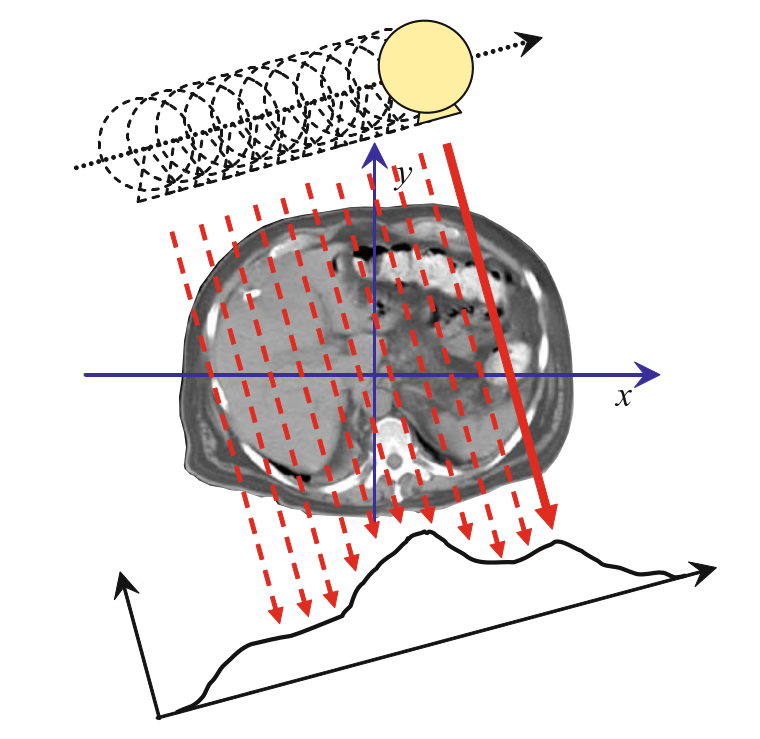
\includegraphics[width=0.58\linewidth]{img/parallel_beam_geometry}%
\label{subfig:parallelbeam}}
\hfil
\subfloat[Fan Beam]{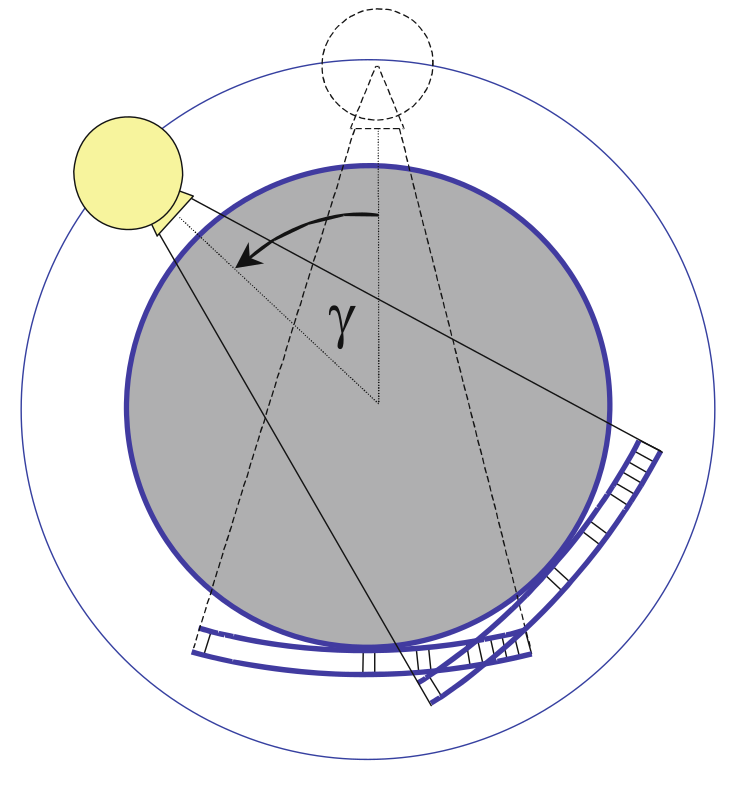
\includegraphics[width=0.4\linewidth, trim=0 -6cm 0 0]{img/fanbeamgeometry}%
\label{subfig:fanbeam}}
\caption{Parallel beam and fan beam geometry. 
In parallel beam the source moving perpendicular to the ray direction for sampling a 1-dimensional image (graph). 
In fan beam, rays are not perpendicular but instead emmited in fan blade form. 
$\gamma$ is the rotation angle at which the signal is obtained. 
Figures from~\cite{Buzug2008_chap3,Buzug2008_chap4}}
\label{fig:parallalandfanbeam}
\end{figure}

This projection geometry can be mathematically expressed with the Radon transform.
When we think of the object as a function of attenuation coefficients $f(x,y)$ and the measured signal as a function of projected coefficients $R(r,\gamma)$ where $r$ is the position on the detector and $\gamma$ is the rotation angle at which the signal is obtained, then
\begin{equation}
\label{eq:radon}
R(r,\gamma) = \int_{-\infty}^{\infty} f(r\;cos(\gamma) + t\;sin(\gamma), r\;sin(\gamma)-t\;cos(\gamma))\;dt.
\end{equation} 
The parameter $t$ is the position on the ray that hits the detector at $r$ and angle $\gamma$, which makes it clear that the projection $R(r,\gamma)$ is the integral along a ray through the object $f(x,y)$.
The sampling of an object in this fashion, results in a so called sinogram.
The contribution of a specific area of the object to the individual projections, follows a sinusoidal path along the $\gamma$-axis as can be seen in \cref{fig:sinogram_parallel}
%
\begin{figure}[!h]
\centering
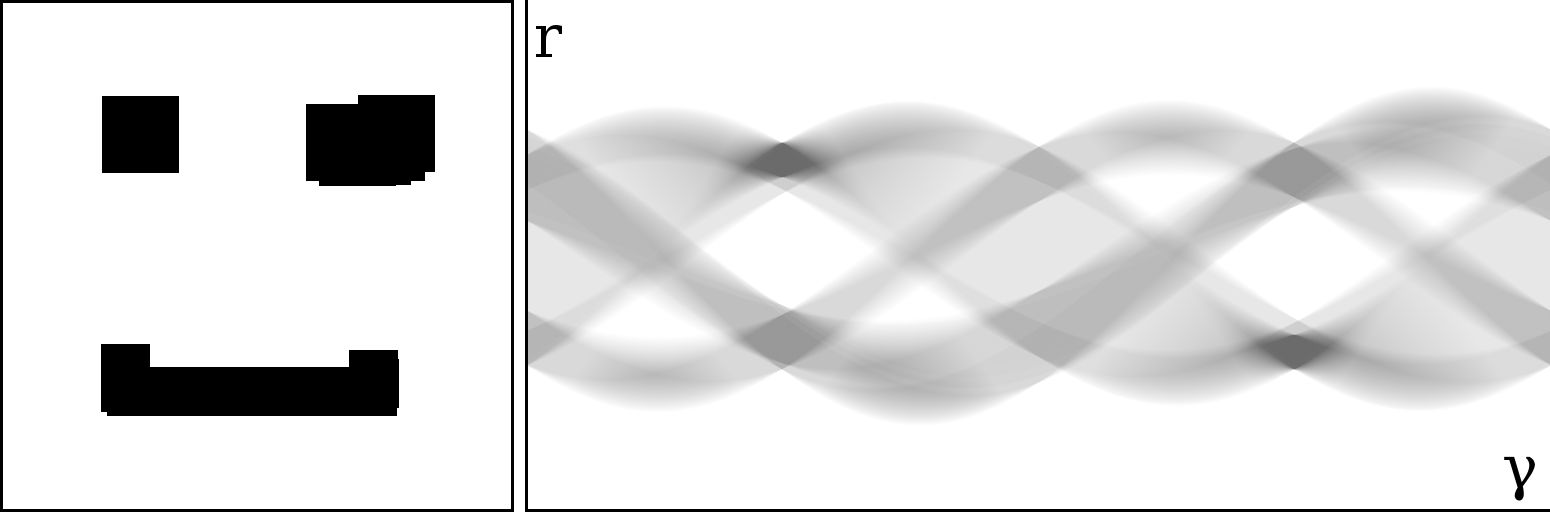
\includegraphics[width=\linewidth]{img/phantomandradon.png}
\caption{
A \enquote{smilie} phantom and its corresponding sinogram with $\gamma~\in~[0^\circ,360^\circ]$.
An imaginary CT would have started with source on top and detector on bottom and then rotated clockwise around the phantom to obtain the shown sinogram.
}
\label{fig:sinogram_parallel}
\end{figure}
%

Unfortuantely, parallel beam geometry is impractical as a pencil beam \xray source (source emmiting only one ray in a specific direction) would have to be moved parallel to the detector to collect all samples for a single rotation angle, which is very time consuming \cite{Buzug2008_chap7}.
However, parallel beam geometry occurs at synchrotron facilities \cite{something}.

\subsubsection{Fan Beam}
A more practical geometry is the fan beam, in which a source emits a flat beam that extends to the sides (like a fan blade). 
\Cref{subfig:fanbeam} shows a schematic of this geometry.
Here the projection for a single rotation angle can be obtained at once. 
The geometry can be defined by the COR it rotates around, the offset of the source to the COR and its aperture angle.
In clinical practise curved detector rays are used, as shown in \cref{subfig:fanbeam}, to get constant aperture angle steps for each detector cell.
%
\begin{figure}[!h]
\centering
\subfloat[]{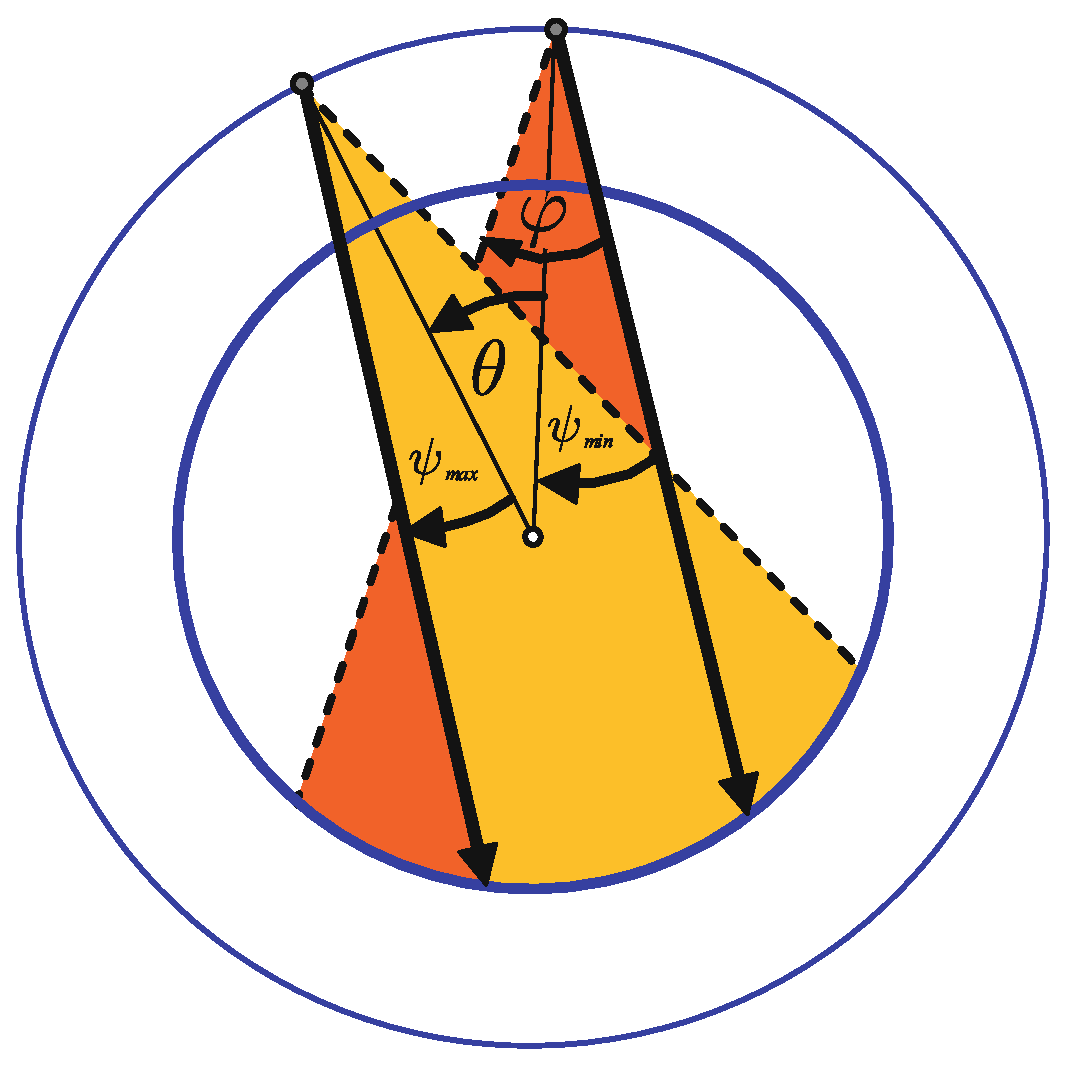
\includegraphics[width=0.43\linewidth]{eps/rebinning.eps}%
\label{subfig:rebinning1}}
\hfil
\subfloat[]{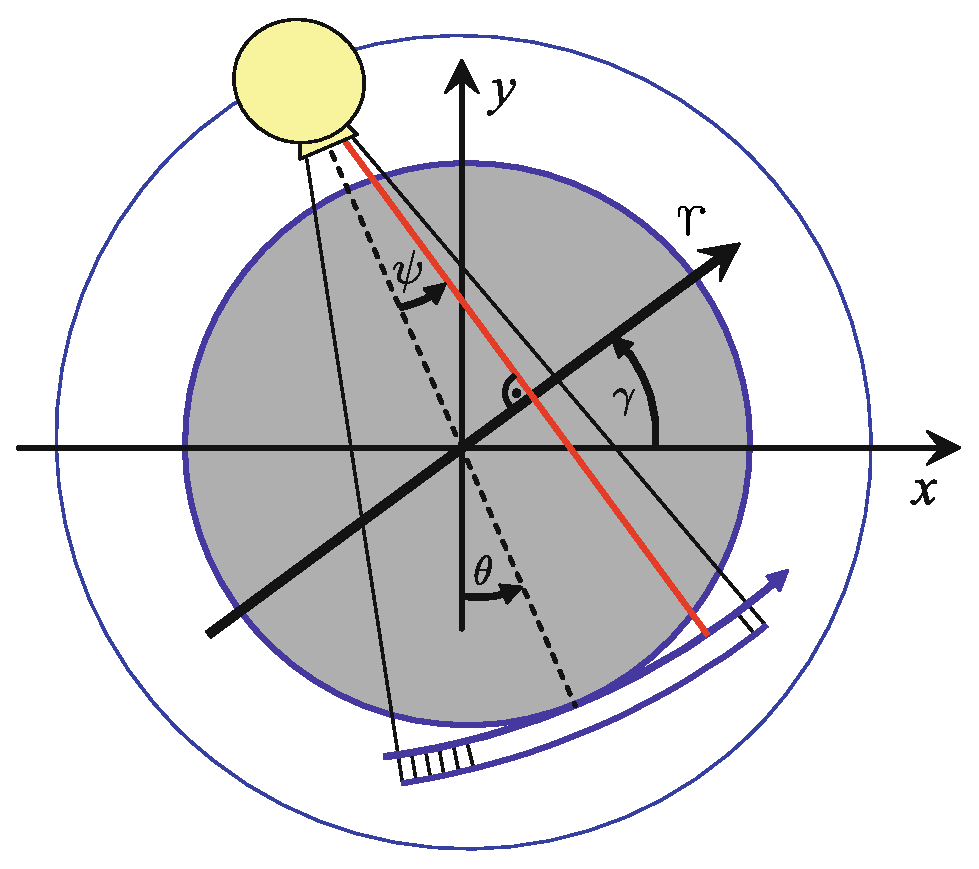
\includegraphics[width=0.51\linewidth]{eps/rebinning_geo.eps}%
\label{subfig:rebinning2}}
\caption{
On the left a schematic is shown with two fan beams with aperture angle $\varphi$ at different rotation angles.
It can be sen that the outer rays of the two are parallel.
The maximum distance of two parallel beams is limited by $\varphi$, and the maximum rotation angle $\theta$ at which two
parallel rays can be obtained is given by $\theta = \psi_{min}+\psi_{max}$ which are the angles from central to outer rays.
On the right a schematic is shown that points out the correspondence between fan and parallel beam geometry.
It can be seen that for the red ray which is the ray at rotation angle $\theta$ with deviation angle $\psi$ from the central ray, there exists an angle $\gamma$ in parallel beam geometry so that it is perpendicular to the $r$-axis (i.e. parallel beam detector).
Figures from~\cite{Buzug2008_chap7}
}
\label{fig:rebinning}
\end{figure}
%

As each ray projection for a single rotation angle in this geometry corresponds to a different ray directions (i.e. rays are not parallel here), the resulting sinogram differs from the sinogram of parallel beam geometry.
When analyzing this geometry further, it can be seen that the ray projections of a parallel beam geometry are inherent and can be found at different rotation angles.
Through a process called rebinning, the sinogram of the fan beam can be transformed to parallel beam.
\Cref{fig:rebinning} illustrates this concept.
 

\subsubsection{Cone Beam}
The previously introduced geometries are both 2-dimensional (2D) as they described projections within an x-y-plane onto a one dimensional detector.
To obtain a 3-dimensional (3D) image the scanned object would have to be moved perpendicular to the plane to obtain multiple slice images.
With the 3D cone beam geometry, this is not necessary as it uses a cone shaped beam that projects onto a 2D flat panel detector.
%
\begin{figure}
\centering
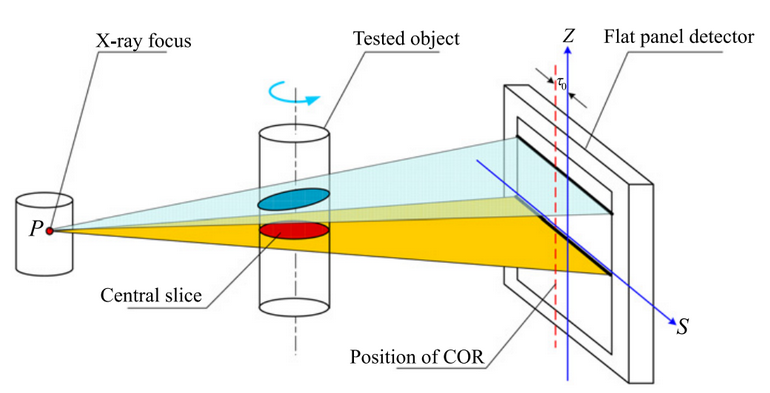
\includegraphics[width=\linewidth]{img/conebeam_centralslice.png}
\caption{
A cone beam setup with an object on a rotary table.
It can be seen that only the projection of the central slice is equivalent to a projection in fan beam geometry.
Other projections that are parallel to the s-axis of the detector use samples at multiple heights of the object.
Also the projection of the rotation axis onto the detector is shown which in this case is offset from detectors
z-axis.
Figure from \cite{Yang2011}
}
\label{fig:conebeam}
\end{figure}
%
In \cref{fig:conebeam} it can be seen that there exists a certain line on the detector which will receive the same input as a fan beam detector.
All other lines read projections through multiple planes of the object and are thus not rebinnable to parallel beam.


\subsection{Reconstruction}
This subsection will explain the process of reconstructing an image from the projections obtained in CT.
Only the 2D case will be explained as it is relevant for understanding the COR determination techniques later on.
Also this subsection will only cover Fourier based reconstruction, especially filtered back projection.

The problem of reconstruction can be stated as follows.\\
Given the Radon transform from \cref{eq:radon} $R(r,\gamma)$ how do we calculate the original signal $f(x,y)$?
The solution to this would be the inverse Radon transform $R(r,\gamma)^{-1}$.
To solve this, the Fourier slice theorem can be leveraged.
%
\begin{align}
p(x) &= R(x,0) = \int_{-\infty}^{\infty} f(x,y)\;dy. 
\\
\hat{f}(u,v) &= \int_{-\infty}^{\infty}\int_{-\infty}^{\infty}f(x,y)e^{-2\pi i (xu+yv)}\;dx\;dy.
\\
s(u) &= \hat{f}(u,0) = \int_{-\infty}^{\infty}\int_{-\infty}^{\infty}f(x,y)e^{-2\pi i xu}\;dx\;dy
\label{eq:fourierslice}
\\
&= \int_{-\infty}^{\infty}\left[\int_{-\infty}^{\infty}f(x,y)\;dy\right]\;e^{-2\pi i xu}\;dx
\nonumber
\\
&= \int_{-\infty}^{\infty}p(x)e^{-2\pi i xu}\;dx = \hat{p}(u).
\nonumber
\end{align}
%
The proof of the Fourier slice thoerem above (\cref{eq:fourierslice}) states that the Fourier transform $\hat{p}(u)$ of a projection $p(x)$ of $f(x,y)$, is the same as the slice $s(u)$ (parallel to the projection line and through the center) of the Fourrier transform $\hat{f}(u,v)$ of $f(x,y)$.
In short $s(u) = \hat{p}(u)$.

As th Radon transform is a set of projections the Fourier slice theorem can be used to build the Fourier tranform of the original signal and reconstruct it using the inverse Fourier transform.
\Cref{fig:inverseradon} illustrates this method.
%
\begin{figure}[!h]
\centering
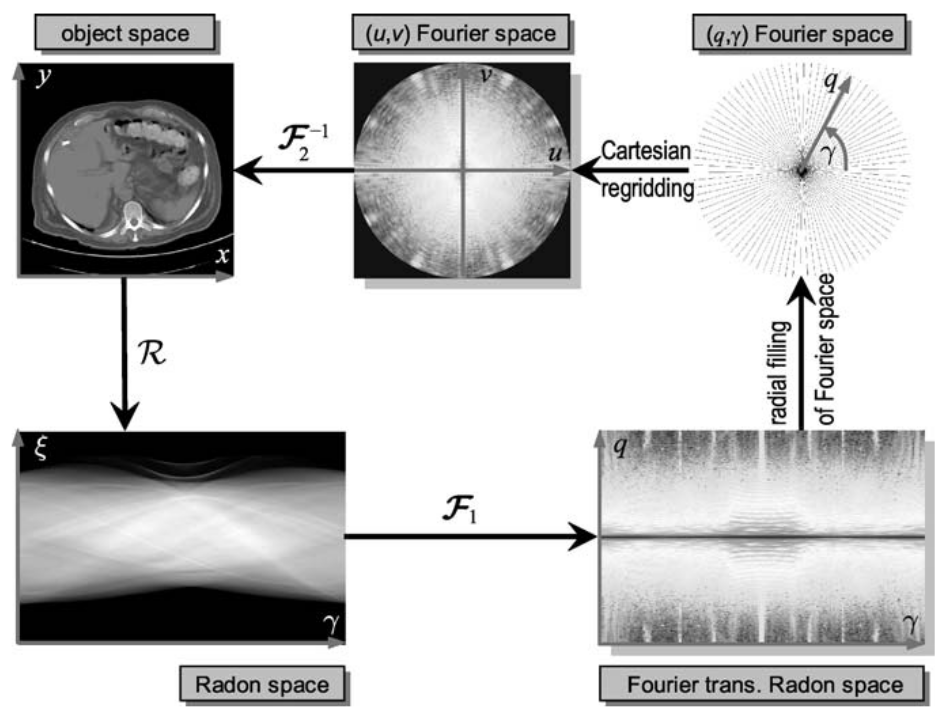
\includegraphics[width=\linewidth]{img/inverseradon.png}
\caption{
The inverse Radon transform can be calculated using the Fourier slice theorem.
First all projections are transformed to the Fourier space along the $\xi$-axis ($=r$-axis).
Then the Fourier transform is built by placing all transformed projections according to their angle into a polar coordinate system.
The coordinate system thus consists of slices of the Fourier transform of the original signal which can then
be obtained using an inverse Fourier transform.
Figure from \cite{Buzug2008_chap5}
}
\label{fig:inverseradon}
\end{figure}
%
The problem of applying this algorithm in practise is, that due to the limited angular resolution (i.e. discretization) of the Radon transform the frequency information density in the Fourier space decreases for higher frequencies \cite{Buzug2008_chap5}.
In the process of cartesian regridding of the polar coordinates a lot of data for the high frequencies would have to be made up in order to perfrom an inverse fast fourier transform.
Therefore a different algorithm, the filtered back projection, is used in practise.

\subsubsection{Filtered Back Projection}
The back projection algorithm reconstructs the original image from a discrete radon transform (i.e. parallel beam sinogram).
For the reconstruction of a single pixel, the information has to be gathered from the ray projections of the rays that intersect this pixel (see \cref{eq:backprojection}).
\begin{equation}
\label{eq:backprojection}
g(x,y) = \int_0^\pi R(x\;cos(\gamma)+y\;sin(\gamma),\gamma)\;d\gamma. 
\end{equation}

This can be imagined as smearing the projections over a canvas in their respective directions.
At first glance this may seem as the correct inversion of the projections but is not.
This becomes clear when thinking about the original image being a dirac delta (image with all entreis zero except for the central pixel).
The projections of this image will be 1D dirac deltas, but using the back projection algorithm will not
restore the 2D dirac but instead smear the 1D diracs also into areas which are supposed to be zero.
In fact the resulting image looks quite blurry which is due to the back projection equaling to the original image convolved with the point spread function of the imaging system (i.e. the Radon transform) $\frac{1}{|(x,y)|}$ \cite{Buzug2008_chap5}.
To counter this, the projections first need to be filtered with a high pass filter.
This introduces negative values in the projections which in the back projection process cancel out positive contributions of other projections.
Figure \cref{fig:backprojection} shows the results of unfiltered and filtered back projection.
As amplifying high frequencies also aplifies noise, there are different filters that can be used in practise \cite{farquhar1998}.
%
\begin{figure}[!h]
\centering
\subfloat{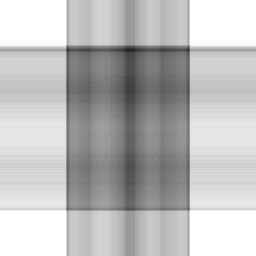
\includegraphics[width=0.18\linewidth]{img/bp_02}}
\hfil
\subfloat{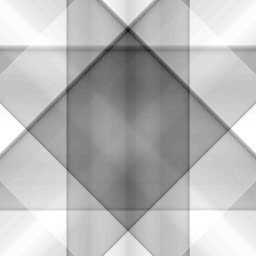
\includegraphics[width=0.18\linewidth]{img/bp_04}}
\hfil
\subfloat{
\includegraphics[width=0.18\linewidth]{img/bp_08}}
\hfil
\subfloat{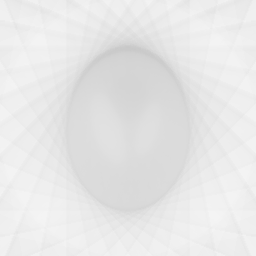
\includegraphics[width=0.18\linewidth]{img/bp_16}}
\hfil
\subfloat{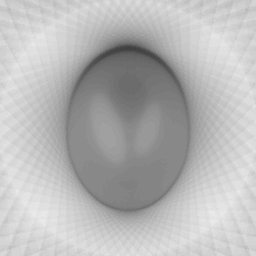
\includegraphics[width=0.18\linewidth]{img/bp_32}}
\\
\subfloat{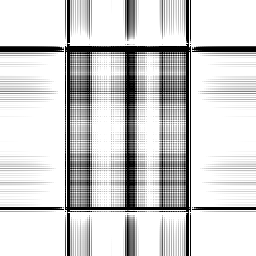
\includegraphics[width=0.18\linewidth]{img/fbp_02}}
\hfil
\subfloat{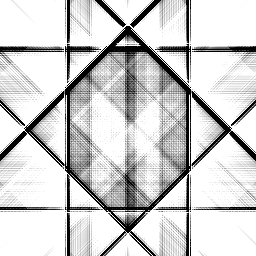
\includegraphics[width=0.18\linewidth]{img/fbp_04}}
\hfil
\subfloat{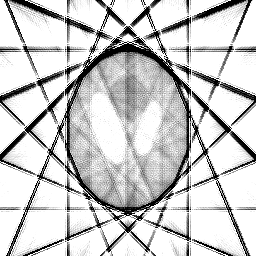
\includegraphics[width=0.18\linewidth]{img/fbp_08}}
\hfil
\subfloat{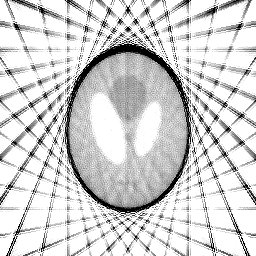
\includegraphics[width=0.18\linewidth]{img/fbp_16}}
\hfil
\subfloat{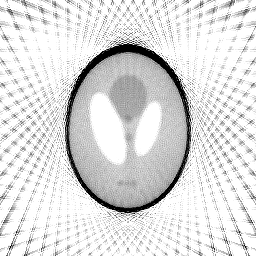
\includegraphics[width=0.18\linewidth]{img/fbp_32}}
\caption{
On the top row, the results of unfiltered back projection are shown. 
From left to right the number of projections used increases from 2 to 32.
The resulting image looks blurry.
On the bottom row the results of filtered back projection are shown.
The resulting image looks quite crips and edges are clearly visible.
The Shepp Logan phantom~\cite{shepplogan} was used as source image.  
}
\label{fig:backprojection}
\end{figure}
%


\section{COR Determination}
The problem of incorrect assumption of the location of the COR can occur in CT setups with misaligned source and detector.
Especially in industrial CT with resolutions on the micrometer scale, calibrating a CT system correctly can be very challenging.
In parallel beam geometry, a misaligned COR, i.e. the COR is projected onto $\tau$ on the $r$-axis, results in a shift of the sinogram along the $r$-axis by $\tau$.
\begin{equation}
\label{eq:radonoffset}
R_\tau(r,\gamma) = R(r-\tau,\gamma)
\end{equation}
The actual problem arises when reconstructing the signal from $R_\tau$ as the algorithms, e.g. filtered back projection (FBP), assume the COR to be in the center.
Thus, ray intersections do not lign up correctly and the reconstructed image suffers from streaking artifacts.
\Cref{fig:shiftfbp} shows the effect of shift of COR in FBP.
%
\begin{figure}[!h]
\centering
\subfloat[$\tau=0$px]{
\includegraphics[width=0.24\linewidth]{img/fbp_shift_0}}
\hfil
\subfloat[$\tau=2$px]{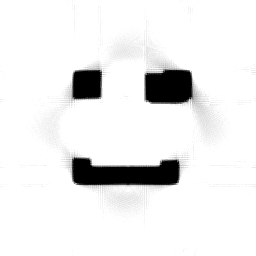
\includegraphics[width=0.24\linewidth]{img/fbp_shift_2}}
\hfil
\subfloat[$\tau=4$px]{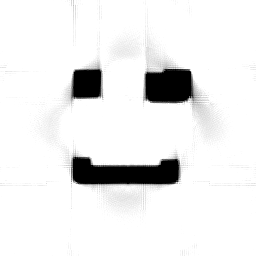
\includegraphics[width=0.24\linewidth]{img/fbp_shift_4}}
\hfil
\subfloat[$\tau=8$px]{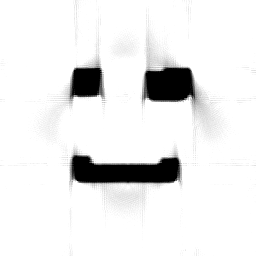
\includegraphics[width=0.24\linewidth]{img/fbp_shift_8}}
\caption{
FBP of the phantom from \cref{fig:sinogram_parallel} with different shifts ($\tau$) of COR.
The resolution of the sinogram in $r$ direction was 256 pixels.
With incresing shift, stronger vertical streaking artifacts are introduced into the reconstructed image.
}
\label{fig:shiftfbp}
\end{figure}
%

In order to correctly reconstruct the signal, the COR first need to be determined.
Several approaches to this problem can be found in the literature, which will be introduced in the following subsections.
The variety of approaches can subdivided in sinogram base methods, which analyze a sinogram in order to find the COR, and reconstruction based methods, which compare reconstruction results with different COR in an iterative fashion.

\subsection{Sinogram Based Methods}
In this subsection the approaches that are based on sinogram analysis are introduced.
The approaches are presentred in chronical order.

\subsubsection{High Density Feature}
Crawford~et~al.~\cite{crawford1988} presented an approach for finding the COR in which they used two $180^\circ$ opposing projections of a distinct high density feature.
When locating this feature in the two projections, the COR can be calculated as the sum of the detector coordinates of the feature divided by two.
This becomes clear when thinking about the feature being offset from the COR by $\delta$ in projection $p_1$.
The corresponding position of the feature in projection $p_2$ will then be on the opposite side of the COR, offset by $-\delta$ from the COR. \Cref{fig:highdenistyfeature} illustrates this concept.
%
\begin{figure}[!h]
\centering
\subfloat[phantom]{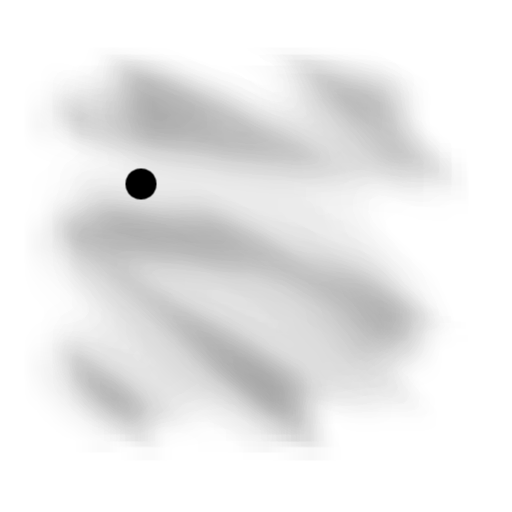
\includegraphics[width=0.32\linewidth]{img/highdensity_inv.png}}
\hfil
\subfloat[sinogram]{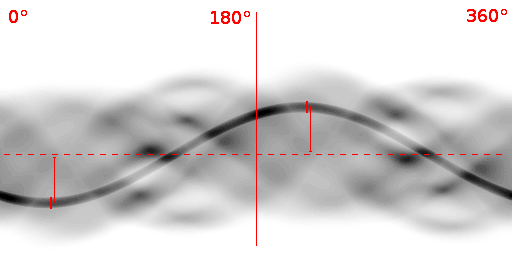
\includegraphics[width=0.65\linewidth]{img/highdensityradon_degrees_feature_centerline_horiz.png}}
\caption{
A phantom with a high density feature is shown on the left side.
In corresponding sinogram on the right, the sinusodial trace of the feature can be observed.
The dotted line indicates the COR in the sinogram.
It can be seen that the feature locations in $180^\circ$ opposing projections have the same distance to the COR.  
}
\label{fig:highdenistyfeature}
\end{figure}
%

This approach could also be expanded to use all projections in the sinogram.
For each opposing pair of projections the COR could be calcualted and then the mean of all CORs will yield the final result.
This approach can be automated if there esists a distinct global maximum in the projections of the sinogram, otherwise a location of the correct feature is not guaranteed.


\subsubsection{Center of Mass}
Azevedo~et~al.~\cite{azevedo90} proposed a more generally applicable algorithm, in which they replaced the high density feature from \cite{crawford1988} with the center of mass.
The center of mass of the original signal is a point $(\overline{x},\overline{y}$) which's coordinates can be calculated as follows (calculation of $\overline{y}$ analogous to $\overline{x}$).
%
\begin{equation}
\overline{x} = \frac{
\int_{-\infty}^{\infty}\int_{-\infty}^{\infty}x\;f(x,y)\;dx\;dy
}
{
\int_{-\infty}^{\infty}\int_{-\infty}^{\infty}f(x,y)\;dx\;dy
}
\end{equation}
%
As the center of mass of the original signal $f(x,y)$ is projected onto the projection center of mass in parallel beam geometry, it can be used as a reference feature.
The projection center of mass is dependent on the projection angle and can be calculated as follows.
%
\begin{equation}
\overline{r_\tau}(\gamma) = \frac{
\int_{-\infty}^{\infty}r\;R_\tau(r,\gamma)\;dr
}
{
\int_{-\infty}^{\infty}R_\tau(r,\gamma)\;dr
}
=
\frac{
\int_{-\infty}^{\infty}r\;R(r-\tau,\gamma)\;dr
}
{
\int_{-\infty}^{\infty}R_(r-\tau,\gamma)\;dr
}
\end{equation}
%
where $R_\tau(r,\gamma)$ is the radon transform with COR offset by~$\tau$ (\cref{eq:radonoffset}).
The previous equation can be simplified to the following.
%
\begin{equation}
\label{eq:projection_centerofmass}
\overline{r_\tau}(\gamma) = \tau + \overline{r}(\gamma) = \tau + \overline{x}\;cos(\gamma) + \overline{y}\;sin(\gamma)
\end{equation}
%
Using linear regression (least squares) the parameters $\tau$, $\overline{x}$ and $\overline{y}$ can be approximated from the matrix notation of \cref{eq:projection_centerofmass}.
%
\begin{equation}
\begin{pmatrix}
1 & cos(\gamma_1) & sin(\gamma_1) \\
\vdots & \vdots & \vdots \\
1 & cos(\gamma_n) & sin(\gamma_n) 
\end{pmatrix}
\cdot
\begin{pmatrix}
\tau \\
\overline{x} \\
\overline{y}
\end{pmatrix}
=
\begin{pmatrix}
\overline{r_\tau}(\gamma_1) \\
\vdots \\
\overline{r_\tau}(\gamma_n)
\end{pmatrix}
\end{equation}
%
Even though $\overline{x}$ and $\overline{y}$ are not needed for a correct reconstruction, it is a neat bonus.


\subsubsection{Cross-Correlation}

\subsection{Reconstruction Based Methods}

\subsubsection{Integral of Negativity}

\subsubsection{Histogram Entropy}

\section{Conclusion}
The conclusion goes here.





% if have a single appendix:
%\appendix[Proof of the Zonklar Equations]
% or
%\appendix  % for no appendix heading
% do not use \section anymore after \appendix, only \section*
% is possibly needed

% use appendices with more than one appendix
% then use \section to start each appendix
% you must declare a \section before using any
% \subsection or using \label (\appendices by itself
% starts a section numbered zero.)
%


\appendices
\section{}


% use section* for acknowledgment
%\ifCLASSOPTIONcompsoc
%  % The Computer Society usually uses the plural form
%  \section*{Acknowledgments}
%\else
%  % regular IEEE prefers the singular form
%  \section*{Acknowledgment}
%\fi


%The authors would like to thank...


% Can use something like this to put references on a page
% by themselves when using endfloat and the captionsoff option.
\ifCLASSOPTIONcaptionsoff
  \newpage
\fi



% trigger a \newpage just before the given reference
% number - used to balance the columns on the last page
% adjust value as needed - may need to be readjusted if
% the document is modified later
%\IEEEtriggeratref{8}
% The "triggered" command can be changed if desired:
%\IEEEtriggercmd{\enlargethispage{-5in}}

% references section

% can use a bibliography generated by BibTeX as a .bbl file
% BibTeX documentation can be easily obtained at:
% http://mirror.ctan.org/biblio/bibtex/contrib/doc/
% The IEEEtran BibTeX style support page is at:
% http://www.michaelshell.org/tex/ieeetran/bibtex/
\bibliographystyle{IEEEtran}
% argument is your BibTeX string definitions and bibliography database(s)
\bibliography{bibliography}
%
% <OR> manually copy in the resultant .bbl file
% set second argument of \begin to the number of references
% (used to reserve space for the reference number labels box)
%\begin{thebibliography}{1}
%
%\bibitem{IEEEhowto:kopka}
%H.~Kopka and P.~W. Daly, \emph{A Guide to \LaTeX}, 3rd~ed.\hskip 1em plus
%  0.5em minus 0.4em\relax Harlow, England: Addison-Wesley, 1999.
%
%\end{thebibliography}




% that's all folks
\end{document}

